\graphicspath{ {./resources/rob/} }
\documentclass[../templateLTHtwocol.tex]{subfiles}
\begin{document}

Assessing the robustness of black box models has always been a challenge. While the control algorithms employing the classical control principles have an empirical to quantify robustness and evaluating performance, quantifying the robustness in the case of black box models relies on deliberate disturbance and adversarial techniques. We resort to the approach of injecting disturbance to evaluate the RL policy and also explore the possibility of improving robustness by subjecting the agent to external disturbance during the training phase. At first glance, it might be reasonable to expect that training with disturbance would make the RL policy more resilient to external disturbances. However, the experimental results refute the assumption. We find the RL agent to have inherent robustness and training with external disturbance did not have a significant impact. Our findings corroborate similar results reported for other continuous control systems \cite{charac_robustness}.

We focus on step/pulse disturbance, as it is more realistic and emulates the wind disturbance experienced by the quadcopter. However, the disturbance is applied in multiple directions (along the XYZ axes). To make it challenging, during the training phase, the direction of the disturbances is switched every few iterations randomly. Figure \ref{rob_ext_dists:fig} shows the training disturbances applied, the disturbance is applied along X, then Z, and then along all three axes XYZ. The evaluation is based on the fixed step disturbances and the performance is measured individually for varying magnitudes of disturbance along individual axes. This also ensures that the replay buffer always contains a good sample.

\begin{figure}[H]
	\centering
	\caption{External Disturbances Applied - Training}
	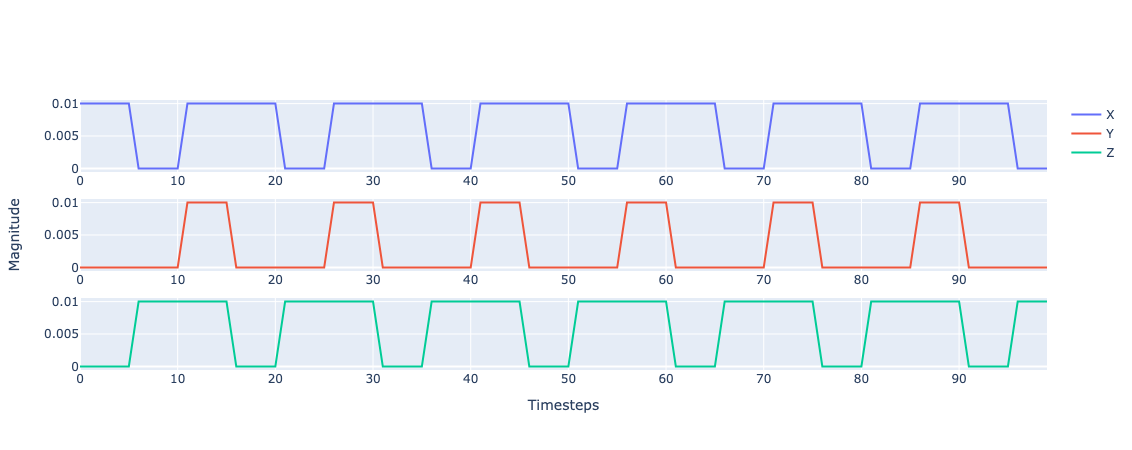
\includegraphics[scale=0.2]{ext_dists.png}
	\label{rob_ext_dists:fig}
\end{figure}

\subsection{Hardware Implementation}

Once the reinforcement learning was done, the actor-network (neural network) was extracted. The real-time inference was achieved by running the model on the computer and sending the actions to CrazyFlie 2.1 over the radio by continuously reading the sensor measurements. The compatibility of states was ensured by reading all of the required measurements from the onboard sensors and converting the quantities to respective units. The position ($[x, y, z]$), orientation ($[r, p, y]$) and linear velocities ($[v_x, v_y, v_z]$) were read from the Kalman filter estimates. And the angular velocities ($[\omega_x, \omega_y, \omega_z]$) were obtained from the gyro.

\end{document}